\chapter{Analysis}

	\section{Quiz Scores}
		There are 4 games with quizzes, each with 30 responses each, 120 responses total. The mean quiz differences were analyzed for statistical significance using a two-tailed t-distribution.

		\subsection{How analysis using a t-distribution works}

			When evaluating statistical significance for paired samples, we have to use a test called a two-tailed t-distribution. More information can be found here \cite{tdist1} and here \cite{tdist2}.

			First, we take our paired samples. For us, these are our pairs of pre-quiz and post-quiz scores for each worker. We find the difference for each pair, which gives us a change for each worker.

			Then, we calculate the mean and standard deviation of these quiz differences. Using either a 90\% or 95\% probability rating, we plug our number of raters, mean, and standard deviation into a two-tailed t-distribution. Increasing the number of samples will tend to reduce the uncertainty limits of the distribution. I used the number of raters minus one as our degrees of freedom.

			The error bars displayed are our confidence limits - we are 90\% or 95\% sure that the true mean lies within these limits. 

			The null hypothesis, that our mean = 0, means that it's possible that our quiz had absolutely no affect. In order to invalidate that hypothesis, and prove that our quiz had a measurable effect, we want the error bars to not be touching zero; that way, the possible true mean cannot equal zero.

		\subsection{Analysis of Quiz Scores using t-distributions}

			\subsubsection{Aggregated}

				\begin{figure}[] 
					\centering 
					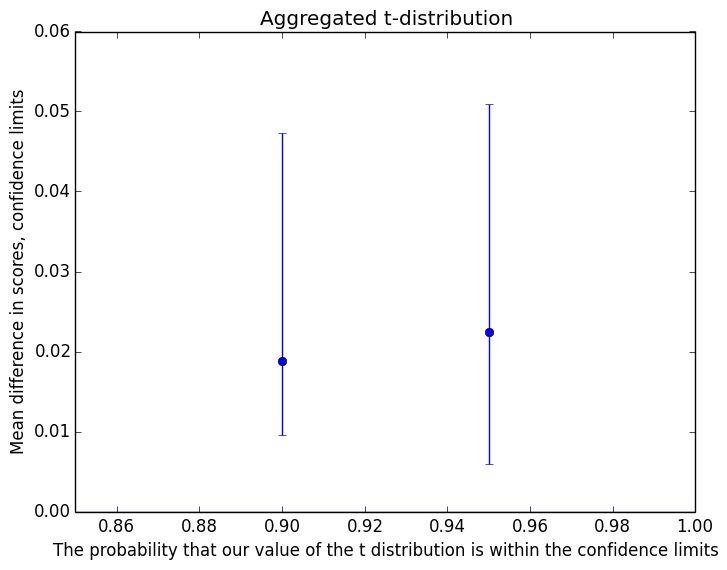
\includegraphics[width=\textwidth, height=.4\textheight, keepaspectratio=true]{aggregated_tdist.png} 
					\caption{Aggregated tdist}
				\end{figure}

				If we aggregate the score differences across all quizzes, our results show that the true mean cannot equal zero, and thus say that our improvement in quiz scores are statistically significant. However, the quiz for each game contains different content and is laid out in a different manner, so we can't use the data aggregated across quizzes.

			\subsubsection{Darfur is Dying}

				\begin{figure}[] 
					\centering 
					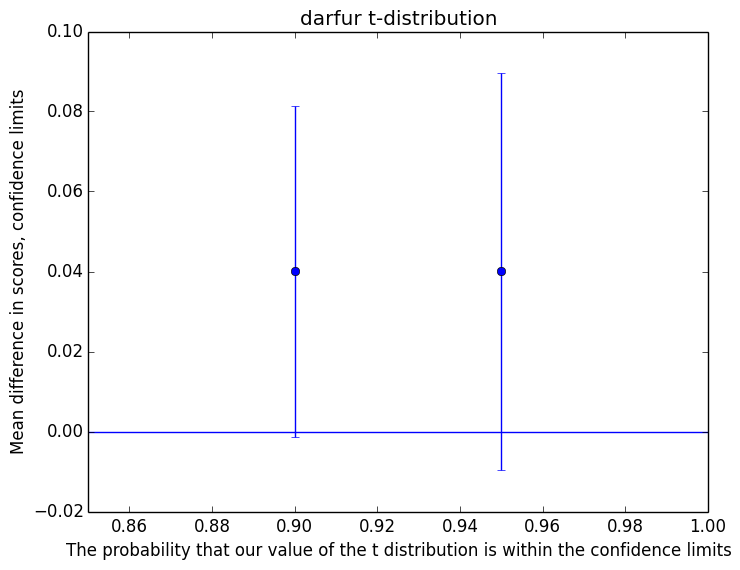
\includegraphics[width=\textwidth, height=.4\textheight, keepaspectratio=true]{darfur_tdist.png} 
					\caption{Darfur tdist}
				\end{figure}

				We cannot eliminate the null hypothesis for our \textit{Darfur is Dying} quiz, even if we reduce the probability to 0.9. This means that our quiz results for \textit{Darfur is Dying} are not statistically significant.

			\subsubsection{The Oregon Trail}

				\begin{figure}[] 
					\centering 
					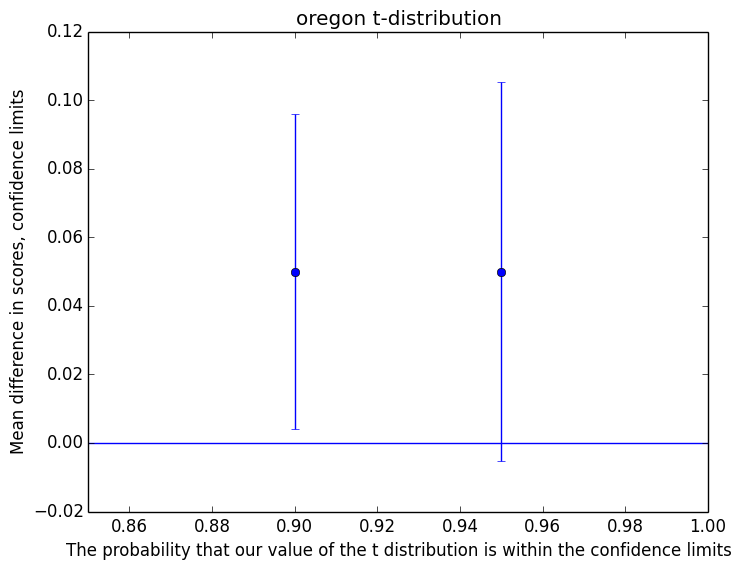
\includegraphics[width=\textwidth, height=.4\textheight, keepaspectratio=true]{oregon_tdist.png} 
					\caption{Oregon tdist}
				\end{figure}

				If we use p = 0.95, we cannot eliminate the null hypothesis for \textit{The Oregon Trail}. However, if we reduce p to 0.9, we can eliminate the null hypothesis, and say that our quiz results for \textit{The Oregon Trail} are statistically significant.

				It's important to note that even if our results are statistically significant, the amount by which they are significant is extremely small; somewhere between a 2\% to 10\% increase in score.

			\subsubsection{Light Bot}

				\begin{figure}[] 
					\centering 
					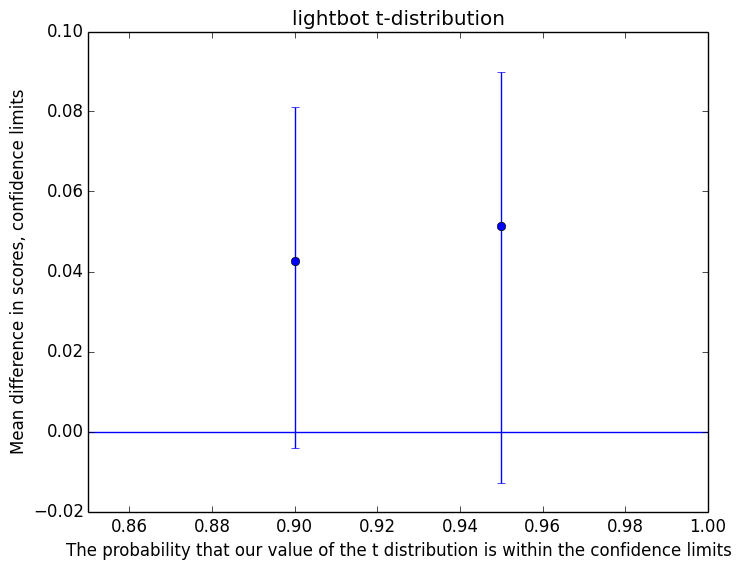
\includegraphics[width=\textwidth, height=.4\textheight, keepaspectratio=true]{lightbot_tdist.png} 
					\caption{Lightbot tdist}
				\end{figure}

				We cannot eliminate the null hypothesis for \textit{Light Bot}, even by reducing p. Our quiz results for \textit{Light Bot} are not statistically significant.

			\subsubsection{Number Munchers}

				\begin{figure}[] 
					\centering 
					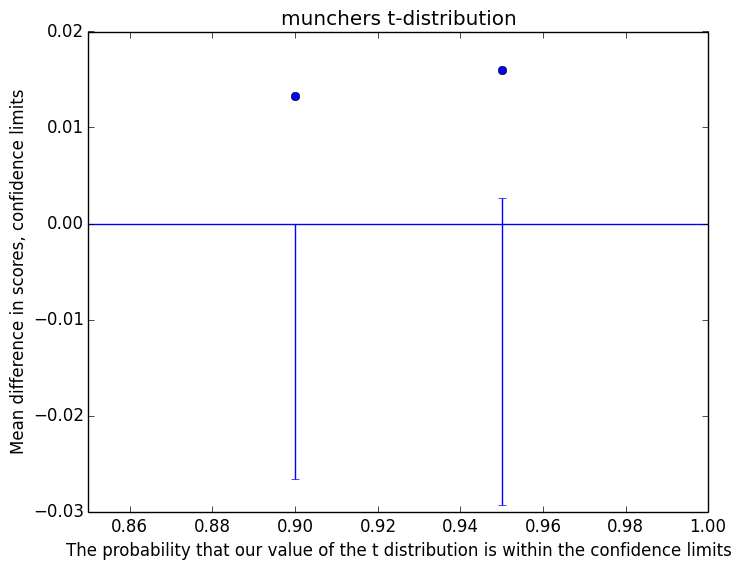
\includegraphics[width=\textwidth, height=.4\textheight, keepaspectratio=true]{munchers_tdist.png} 
					\caption{Munchers tdist}
				\end{figure}

				If we reduce p to 0.9, we can eliminate the null hypothesis from our \textit{Number Munchers} results. However, it's very small, and it's actually in the negative direction; somewhere between a 0\% and 2.5\% decrease in score.

		\section{Rubric Inter-rater Reliability}
			\subsection{How analysis using inter-rater reliability works}

				In order to ensure that the rubric I've built is consistent, we need to measure the responses we recieve using inter-rater reliability. More info can be found here and here.

				Inter-rater reliability gives us a value (kappa) to indicate how consistent a given set of questions are. This is done by getting the results from several workers answering the questions, then analyzing how much they agreed on their responses.

				For example, let's say I had a quiz with 50 True/False questions. If I had 2 people take the quiz, and they each got every single question correct (e.g. they agreed on every single question), the quiz would have a kappa value of 1, perfect agreement. If only one person got every single question correct, and the other got 0 questions correct (e.g. they disagreed on every single question), then the quiz would have a kappa value of -1, perfect disagreement. The values in between 1 and -1 indicate various levels of agreement, with 0 being complete randomness.

				From Landis and Koch \cite{benchmarks}, here are the typical benchmarks for inter-rater reliability.

				\paragraph{-1.0} Perfect Disagreement

				\paragraph{-1.0 to -0.8} Almost Perfect Disagreement

				\paragraph{-0.8 to -0.6} Substantial Disagreement

				\paragraph{-0.6 to -0.4} Moderate Disagreement

				\paragraph{-0.4 to -0.2} Fair Disagreement

				\paragraph{-0.2 to 0.0} Slight Disagreement

				\paragraph{0.0} Completely random

				\paragraph{0.0 to 0.2} Slight Agreement

				\paragraph{0.2 to 0.4} Fair Agreement

				\paragraph{0.4 to 0.6} Moderate Agreement

				\paragraph{0.6 to 0.8} Substantial Agreement

				\paragraph{0.8 to 1.0} Almost Perfect Agreement

				\paragraph{1.0} Perfect Agreement

				\paragraph{}We want to use inter-rater agreement to evaluate the consistency of our design rubric. We'll use the method to evaluate multiple subjects with multiple raters and multiple-choice questions. Instead of looking at the design rubric as a whole document, we can actually examine each rubric item individually, and look at the responses it received across all games.

				Think of it as if we are evaluating 13 different quizzes, one for each design rubric item. On each quiz, there are 10 questions, one for each game to be evaluated. Each question has 5 single-selection options, where each option corresponds to a level on the scale of the rubric item.

				For each graph, each bar indicates a rubric item, with it's height above or below the x-axis indicating its kappa value (up to +1.0 for agreement, up to -1.0 for disagreement).

			\subsection{Analysis for Rubric items using inter-rater reliability}
				\begin{figure}[] 
					\centering 
					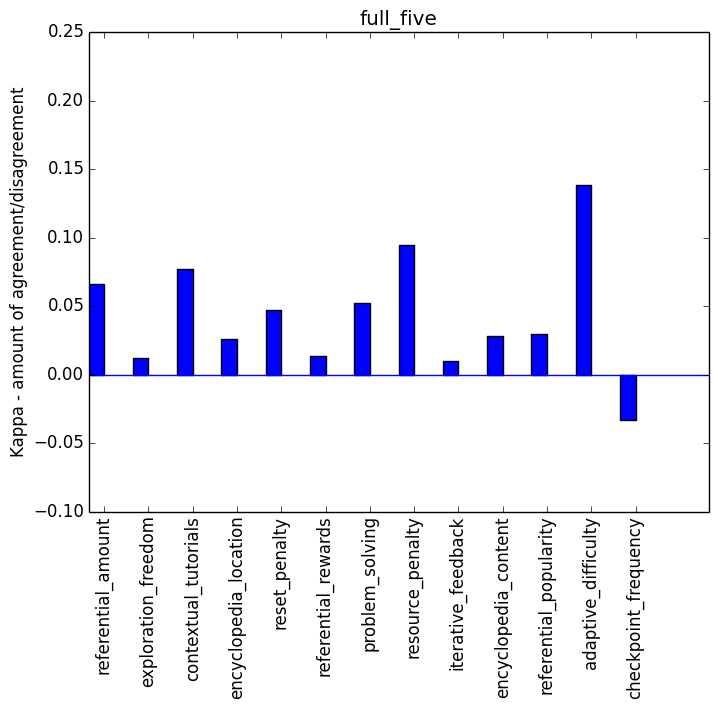
\includegraphics[width=\textwidth, height=.4\textheight, keepaspectratio=true]{full_five_stats.png} 
					\caption{Inter-rater reliability}
				\end{figure}

				The kappa values for each rubric item were very small. All but one of the rubric items fell in the ``Slight Agreement'' category, with Adaptive Difficulty being the highest with a kappa value of 0.15. Checkpoint Frequency was the only negative rubric item. 

				This was unexpected and disappointing. After some further consideration, I decided to process the data slightly differently, to see if it would give me a different result.

				Inter-rater reliability metrics commonly depend on a low number of available options (2 to 3) for workers to choose when taking a quiz. In our above example, our 50 question True/False quiz only contained 2 options for workers to choose from on each question; the rubric that we gave our workers contained 5 options for each question.

				In order to achieve a different result, I ran two additonal inter-rater reliability calculations. With one, I summed the outside pairs together (e.g. [1, 2, 3, 4, 5] became [sum(1, 2), 3, sum(4, 5)]) to give us a result with only 3 choices that workers chose from. For the other calculation, I summed the inner 3 choices(e.g. [1, 2, 3, 4, 5] became [1, sum(2, 3, 4), 5]), to again give a result with only 3 choices.

				\begin{figure}[] 
					\centering 
					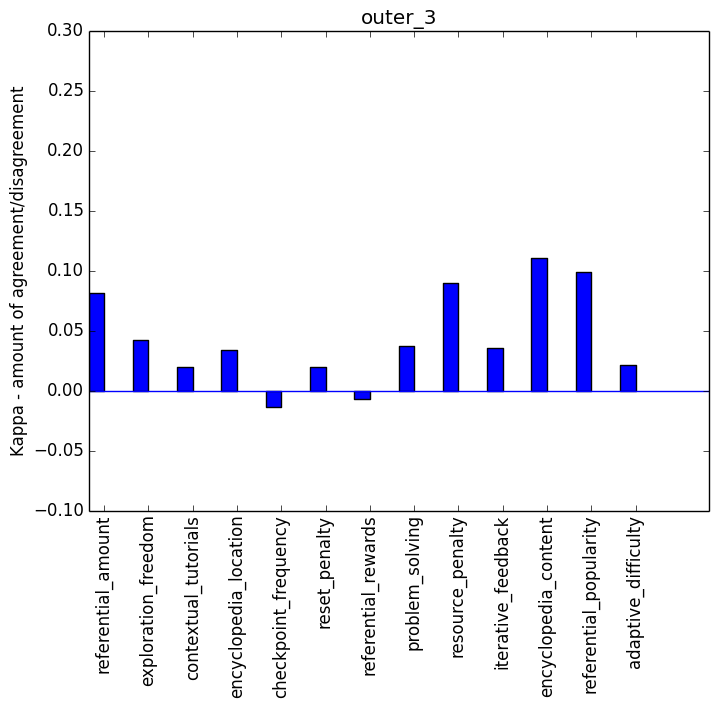
\includegraphics[width=\textwidth, height=.4\textheight, keepaspectratio=true]{outer_3_stats.png} 
					\caption{Inter-rater reliability with outer pairs combined}
				\end{figure}
				\begin{figure}[] 
					\centering 
					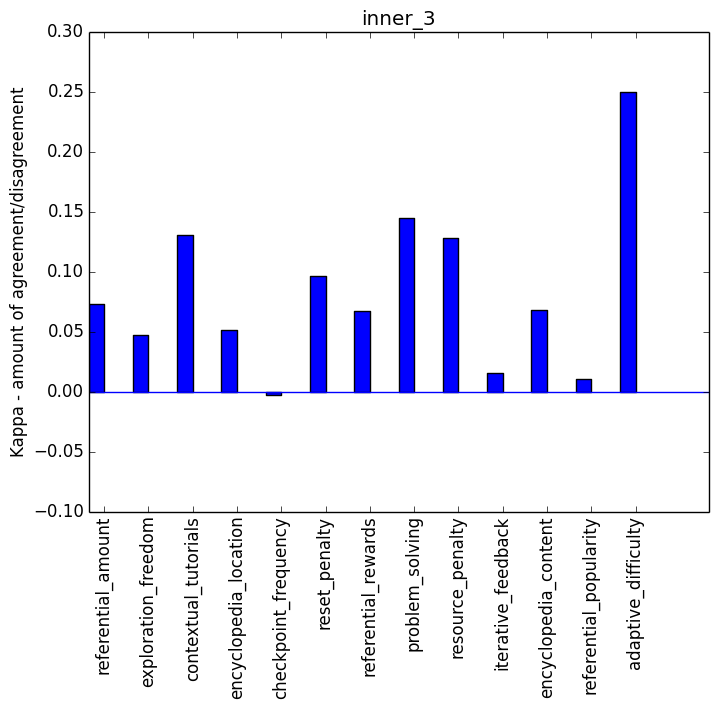
\includegraphics[width=\textwidth, height=.4\textheight, keepaspectratio=true]{inner_3_stats.png} 
					\caption{Inter-rater reliability with middle 3 options combined}
				\end{figure}

				Summing the outer pairs of options doesn't change our scores significantly, but summing the inner scores does. By considering the middle 3 options as a single option, Adaptive Difficulty reaches the ``Fair Agreement'' category with a kappa value of 0.25. Contextual Tutorials, Unorthodox Problem-solving, and Game Resource Penalty all still fall in the ``Slight Agreement'' category, but they have improved kappa values of above 0.10.
				
			













